\cleardoublepage
\chapter{FRAGMENTASI ARSITEKTUR PER PERAN}
\label{appx:fragmentasi-peran}

Lampiran ini menyajikan rincian fragmentasi arsitektur DataOps dan MLOps pada empat peran utama yang dirujuk dari Subbab~\ref{subsec:efek-domino-fragmentasi}. Pembahasan pada bab tersebut diringkas pada pandangan umum agar fokus tetap pada tiga sumber tekanan, yaitu beban konfigurasi platform dari nol, biaya berlangganan layanan terkelola, dan efek domino fragmentasi lintas peran. Detail per peran disajikan di sini sebagai bukti pendukung pemetaan kondisi saat ini.

\section{Fragmentasi pada Peran \textit{Business User}}
\label{appx:fragment-busus}

Peran \textit{business user} biasanya berinteraksi dengan tumpukan visualisasi dan pelaporan yang terpisah dari sumber data analitik dan model. Gambar~\ref{fig:fragment-busus} memperlihatkan posisi peran ini pada arsitektur fragmentasi dengan akses utama melalui \textit{dashboard} dan laporan. Konsekuensinya, informasi tentang metrik \textit{drift}, kualitas data, dan kebijakan akses sering tidak tersaji dalam satu antarmuka, sehingga keputusan bisnis mengandalkan ringkasan berkala yang tidak selalu terhubung dengan kondisi sistem terkini.

\begin{figure}[H]
    \centering
    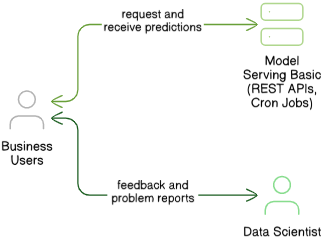
\includegraphics[width=0.85\textwidth]{figures/Fragment_BusUs_Arch.png}
    \caption{Fragmentasi pada Peran \textit{Business User}}
    \label{fig:fragment-busus}
\end{figure}

\section{Fragmentasi pada Peran \textit{Data Engineer}}
\label{appx:fragment-dateng}

\textit{Data engineer} bertanggung jawab atas ingestasi, pemrosesan, dan penyimpanan data. Gambar~\ref{fig:fragment-dateng} memperlihatkan luasnya cakupan tugas pada lapisan ingestasi, transformasi, dan tata kelola. \textcite{lamer2024data} menyoroti kompleksitas tata kelola data yang sering muncul ketika \textit{tool} ingestasi, kualitas, dan katalog tidak terintegrasi pada satu sumber kebenaran. Akibatnya, kebijakan kualitas dan \textit{lineage} antar lapisan data harus disinkronkan secara manual.

\begin{figure}[H]
    \centering
    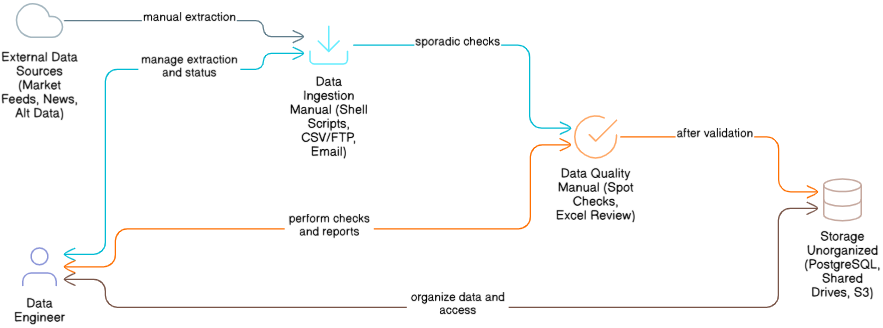
\includegraphics[width=0.85\textwidth]{figures/Fragment_DatEng_Arch.png}
    \caption{Fragmentasi pada Peran \textit{Data Engineer}}
    \label{fig:fragment-dateng}
\end{figure}

\section{Fragmentasi pada Peran \textit{Data Scientist}}
\label{appx:fragment-datsci}

Peran \textit{data scientist} menghabiskan sebagian besar waktu pada eksperimen dan rekayasa fitur. Gambar~\ref{fig:fragment-datsci} memperlihatkan ketergantungan pada \textit{notebook}, \textit{experiment tracking}, dan \textit{feature engineering} yang sering berdiri sendiri. \textcite{anaconda2020state} dan \textcite{pimentel2019notebooks} memperlihatkan bahwa reproduksibilitas eksperimen terganggu apabila lingkungan eksekusi, versi data, dan versi kode tidak diatur dalam satu \textit{pipeline} yang sama, dan kondisi ini diperburuk oleh \textit{technical debt} yang khas pada sistem \textit{machine learning} sebagaimana dipetakan oleh \textcite{sculley2015hidden}.

\begin{figure}[H]
    \centering
    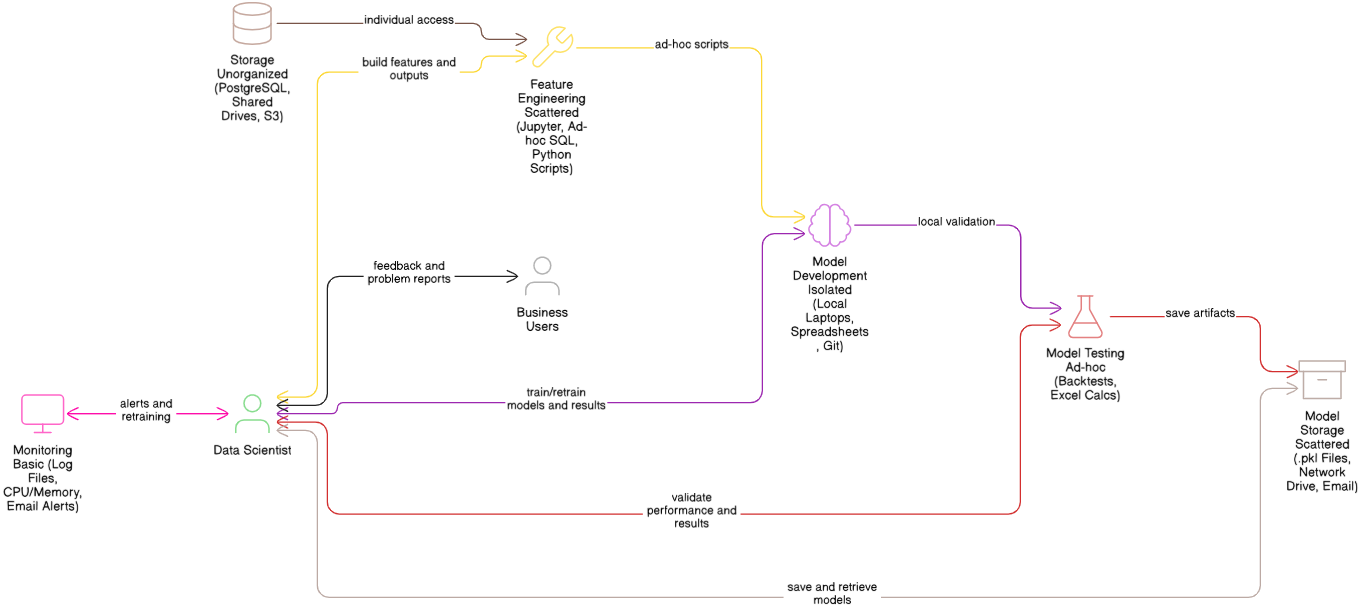
\includegraphics[width=0.85\textwidth]{figures/Fragment_DatSci_Arch.png}
    \caption{Fragmentasi pada Peran \textit{Data Scientist}}
    \label{fig:fragment-datsci}
\end{figure}

\section{Fragmentasi pada Peran \textit{Machine Learning Engineer}}
\label{appx:fragment-mleng}

\textit{Machine learning engineer} bertugas membawa model dari fase eksperimen ke fase produksi. Gambar~\ref{fig:fragment-mleng} memperlihatkan kebutuhan pada \textit{model registry}, \textit{serving}, dan pemantauan model. \textcite{rella2022mlops} memperlihatkan dampak buruk yang muncul ketika siklus hidup model tidak terhubung dengan kontrol versi data dan fitur. Akibatnya, mekanisme \textit{rollback}, \textit{canary}, dan \textit{retraining} tidak konsisten antar tim.

\begin{figure}[H]
    \centering
    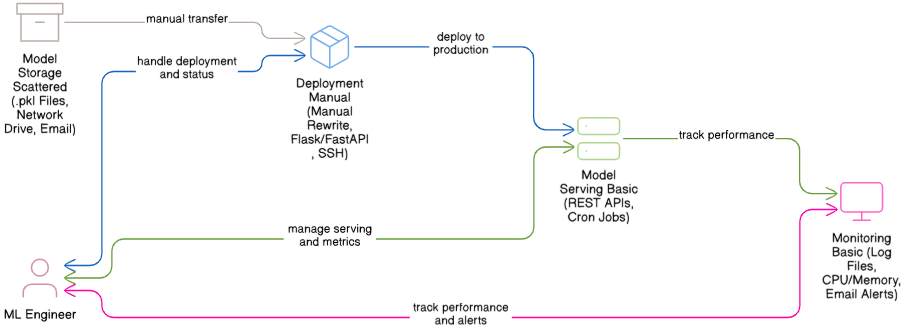
\includegraphics[width=0.85\textwidth]{figures/Fragment_MLEng_Arch.png}
    \caption{Fragmentasi pada Peran \textit{Machine Learning Engineer}}
    \label{fig:fragment-mleng}
\end{figure}
